\begin{frame}{Why do Scripting for GPUs?}
  \begin{columns}
    \column{0.6\textwidth}
    \begin{itemize}
      \item GPUs are everything that scripting languages are not.
        \begin{itemize}
          \item Highly parallel
          \item Very architecture-sensitive
          \item Built for maximum FP/memory throughput
        \end{itemize}
        $\rightarrow$ complement each other
      \item CPU: largely restricted to control tasks ($\sim$1000/sec)
        \begin{itemize}
          \item Scripting fast enough
        \end{itemize}
      \item Python + CUDA = \textbf{PyCUDA}
      \item Python + OpenCL = \textbf{PyOpenCL}
    \end{itemize}
    \column{0.4\textwidth}
      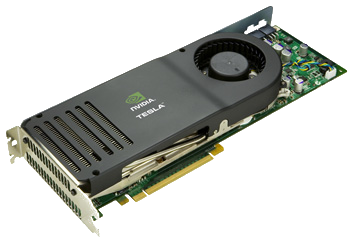
\includegraphics[width=\textwidth]{c870.png}
  \end{columns}
\end{frame}
\addimgcredit{C870 GPU: Nvidia Corp.}

